\documentclass[conference]{IEEEtran}
\usepackage[pdftex]{graphicx}
\graphicspath{{images/}}
\usepackage[backend=biber, style=ieee]{biblatex}
\addbibresource{jprefwolf.bib}
\addbibresource{mwrefwolf.bib}
\usepackage{amsmath} % For better math in tables and equations
\usepackage[final]{microtype} % Makes things look better in the end
\usepackage[hidelinks]{hyperref}

% correct bad hyphenation here
%\hyphenation{op-tical net-works semi-conduc-tor}

\begin{document}
%
% paper title
% Titles are generally capitalized except for words such as a, an, and, as,
% at, but, by, for, in, nor, of, on, or, the, to and up, which are usually
% not capitalized unless they are the first or last word of the title.
% Linebreaks \\ can be used within to get better formatting as desired.
% Do not put math or special symbols in the title.
\title{The Wolf in Sheep's Clothing:\\
Subversive Adversarial Agent Identification}


% author names and affiliations
% use a multiple column layout for up to three different
% affiliations
\author{\IEEEauthorblockN{Jean P. Castillo\IEEEauthorrefmark{1},
Matthew W. Swartwout\IEEEauthorrefmark{2}, Russel C. Jackson\IEEEauthorrefmark{3} and
Murat C. Cavusoglu\IEEEauthorrefmark{4}}
\IEEEauthorblockA{Department of Electrical Engineering and Computer Science,
Case Western Resere University\\
Cleveland, OH 44106\\
Email: \IEEEauthorrefmark{1}jpc87@case.edu,
\IEEEauthorrefmark{2}mws85@case.edu,
\IEEEauthorrefmark{3}rcj33@case.edu,
\IEEEauthorrefmark{4}mcc14@case.edu}}

% conference papers do not typically use \thanks and this command
% is locked out in conference mode. If really needed, such as for
% the acknowledgment of grants, issue a \IEEEoverridecommandlockouts
% after \documentclass

% use for special paper notices
%\IEEEspecialpapernotice{(Invited Paper)}

% make the title area
\maketitle

% As a general rule, do not put math, special symbols or citations
% in the abstract
\begin{abstract}

Mobile robot security is a rapidly developing area of interest in robotics. As mobile robotic systems become more present, the need for secure and reliable state estimation systems continues to grow. The increasing coverage of wireless networks and density of network cyber-physical systems has lead to an opportunity for distributed systems coordinated between multiple agents. This paper proposes a distributed state estimation system using Kalman filters with secure ad-hoc channel communications between the agents. On top of this is a state detection system validation that allows agents to detect subversive or malfunctioning agents in their environment. The detection of such compromised agents can be used to create a trusted set within a group, providing a multi-node trust system. A TurtleBot running Robot Operating System (ROS) platform is used for implementation and performance is also evaluated in the Gazebo simulator.

\end{abstract}

% no keywords


% For peer review papers, you can put extra information on the cover
% page as needed:
% \ifCLASSOPTIONpeerreview
% \begin{center} \bfseries EDICS Category: 3-BBND \end{center}
% \fi
%
% For peerreview papers, this IEEEtran command inserts a page break and
% creates the second title. It will be ignored for other modes.
\IEEEpeerreviewmaketitle

\section{Introduction}
With drones in land, air and sea coming into the growing consumer and private markets, the security involved in groups of these machines must be further studied. Robot security has landed headlines across a variety of commonly used devices, car hacking having a prominent impact in the United States and abroad. Some individuals have been able to remotely connect to, disable, and control various vehicles in the market through techniques like that of Greenber et al, posing many questions about the protocol used in vehicles \cite{greenberg2015hackers}. As more agents become connected, much like cyber-vehicles in a highway would, decisions that each agent makes are based on the information it obtains from not only its sensors but also other agent's data. This paper discusses how an agent can securely obtain the probability that another agent in the system is compromised in order to trust feedback obtained from that agent in question.

There are three core goals for the security of any cyber-physical system: integrity, availability, and confidentiality \cite{Cardenas2008}. Those can be thought of as three simple questions: ``Can I trust the data?'', ``Do I have access to the data when I need it?'', and ``Is the data hidden from those who shouldn't have it?''. In a full trust chain there is an initial block of trust called Hardware Secure Enclosure (HSE) unit which fingerprints specific physical properties of the hardware to uniquely identify an agent. This fingerprint is used to verify various modules of an agent such as the static software, dynamic software, control system and communication of the agent.

Communication between two agents focuses on confidentiality and integrity which can both be accounted for through proper encryption and the data fields inside the encrypted message. A challenge-response system is implemented in this paper which changes, or churns, on every round trip time providing fresh keys for the encrypted payload. The consequence of this design is that every communication is uniquely encrypted, closing doors for leakage of information. Timestamp and source mac address fields inside the encrypted payload ensures not only that the message comes from the individual claiming to be the originator in the raw packet, but also that timing attacks can be properly guarded against. 

Once communication is secured, an adversary can distort the sensor data of an agent in order to lead it in a stray. An agent in the group can detect the abnormality by comparing the state and behavior combination taken to that of an established usage envelope, a term coined here as a pre-computed state trajectory map. This map allows for a large variety of planning algorithms to be used. In light that there is both sensor and mechanical error in the system a Bayes filter is used in order to implement proper weighing of new data coming in.

Redundant measurements in the system allow for an agents inside a trusted set to verify each other's locations. With and without feedback from others in the system, through the use of  several Kalman filters an agent is able to verify the positions of others relative to itself. 

We now relate some work related to integrity, availability, and confidentiality, and further discuss the implementation technique used. 

\section{Related Work}
Chain of trusts, as pertaining to cyber systems, have been introduced in works such as \cite{adi2009mechatronic} where a DNA clone resistant approach is taken throughout; a Physical Unclonable Function (PUF) was introduced which obtains physical differences between other electronic devices. Similar to this work the extended chain of trust this paper is part of a larger work which incorporates a HSE which is used to provide a unique hardware signature used to verify other parts of the system much like \cite{adi2009mechatronic}.

\subsection{State Estimation}
State estimation is a fundamental problem for robotics. Without knowing its location, a robot cannot be very useful. One common technique for robot localization is to use a Kalman Filter (KF). The KF is one of the most studied and most heavily utilized Bayesian filter \cite[39-81]{ProbabilisticRobotics}. At its core, a KF represents the state of a linear system as a multivariate normal distribution. By representing the state of the system as a normal distribution the filter can compactly represent the degree of belief of any possible state of the system.

The application of the KF to the task of robot localization has been studied intently \cite{Localization2003, Mohsin2014}. In \cite{Mohsin2014}, it is explained to be so popular for three main reasons. First, it is optimal under certain reasonable and common assumptions, second that it is recursive which is memory efficient, and finally that it relies only on having knowledge of noisy sensor data and not being able to measure certain state variables directly.

For this paper, we utilize an Unscented Kalman Filter (UKF) for the task of sensor fusion and localization. The UKF provides better accuracy for non-linear systems than a KF or Extended Kalman Filter (EKF) and is less computationally complex \cite{Julier1997}.

\subsection{Secure State Estimation}
Secure State Estimation requires a focus on all three of the previously mentioned facets of security: Integrity, Availability and Confidentiality. We choose to focus on the first and third of these, Integrity and Confidentiality, for our secure estimation system.

\subsubsection{Integrity}
The accuracy of a KF when the sensors are functioning properly is not in question, so we must look at when the sensors are not functioning properly. We propose two primary failure modes for data integrity: sensor failure and false data injection.

In a sensor failure scenario one or more of the sensors will stop providing all feedback. Luckily, this is something that KFs can handle without problem. The KF is always using all available information to generate its state estimate, and if one sensor fails the only result is that the accuracy of the filter will decrease. Obviously, if 100\% of sensors fail, the filter will become non-functional, but as long as at least one sensor remains operational the filter will not have difficulties. It is also worth nothing that, due to the design of the filter, the KF does not have issues with sensors going in and out of a failure state. When information is available it is used, and when it is not available the sensor is ignored.

Knowing that sensor failure is not a huge risk for the KF, sensor interference is a much more complex problem. If an attacker is somehow able to inject false data into the filter the pose estimate can be skewed. And this is a very real problem. The number of ways that false data could be added to a filter are too numerous to count, ranging from physically blocking a lidar sensor to hijacking the network packets of a wirelessly communicating sensor.

\cite{Mo2010} and \cite{Yang2013} both demonstrate that KFs are susceptible to false data injection attacks, and that even with failure detectors a clever adversary can craft their attack to bypass these detectors. \cite{Bezzo_2014} and \cite{Mo2014} both attack this problem by adding extra steps into their KF algorithm. Both successfully show that the filter output can be shielded from the effects of the attack.


\subsubsection{Confidentiality: Secure Ad-Hoc Channel Communication}
There are various works that cover a communications for adhoc networks. \cite{vegh2014securing} uses an extension of the ElGamal algorithm in order to limit the access of agents in the network. In the event that an agent is compromised the information within the decrypted message remains protected through steganography, a method used for hiding information within a text \cite{adi2009mechatronic}. The implementation uses direct agent to agent communication and thus no hierarchy is used; no encrypted broadcast messages are sent and it seems unnecessary to encrypt the information further as it would lead to potential DOS attacks.

Another protocol introduced in \cite{chang2016provably} provides forward secrecy through registration, authentication and password changing involving communication between user, sensor and gateway nodes. A long term secret is used for the session and a change in password occurs once the connection is established; however, in a moving environment there may instances when only two nodes will be able to communicate at one time.

In the field of automobiles \cite{lyu2016pba} developed a protocol named PBA that is well guarded against high traffic and lossy wireless networks. Work in \cite{lyu2016pba} addresses DOS attack resistance and stores shortened MAC address signatures for memory consumption and rapid verification. \cite{lyu2016pba} takes a private public key pair approach which may be prone to further attacks as the base station could update their keys. Connectivity to the central station after the release is not taken to be necessary in this paper's approach.

\subsection{Distributed State Estimation}
As wireless networks become more and more omnipresent in our world, and given the increasing number and decreasing costs of mobile robots, the concept of a distributed state estimation system is very desirable. Given the rapid rise of these technologies though, the amount of research done into distributed systems is quite small compared to that for single robots. This was true years ago (\cite{Parker2000}), and is still true today.

Traditionally, in order to increase the accuracy of state estimation, more sensors are added to a robot. However, increasing the number of sensors on a robot will increase the cost and complexity. And, where a robot operating by itself might need $n$ sensors for a sufficiently accurate state estimate, when operating in an environment surrounded by $m$ other robots that can share sensor data there is the possibility of needing far fewer sensors on each individual robot.

Most research into such distributed systems relies on the concept of cooperative positioning. That is, the robots coordinate their motions in order to use their sensors to determine the state of the other robots. Most often this involves one robot acting as a stationary landmark while the other robot moves. \cite{Kurazume1994}, \cite{Kurazume1996}, \cite{Kurazume1998}, and \cite{Kurazume2000} all explore the idea of cooperative positioning. This is a valuable and effective concept when working with a team of coordinated robots. However many systems will not allow for such close cooperation. For example, autonomous cars on a highway will not be able to start and stop for each other and still get to their destination on time. And in rush hour in a city the processing power needed to coordinate a plan for the thousands of cars on the road would be incredible.

Other work into distributed systems still makes the assumption of a cooperative team. \cite{Sanderson1997} and \cite{Roumeliotis2002} both demonstrate a system where a KF is implemented that estimates the state of multiple robots in a system. However these states are computed relative to each other, considering the network of robots to be essentially one large robot with different parts. Continuing the highway example, cars will be moving in and out of communication with each other as some enter the highway and others exit. Thus the group of robots will be constantly changing and evolving, a challenge not tackled by these works.

The previously mentioned works are all examples of a decentralized, rather than distributed KF problem. \cite{Olfati-Saber2005} makes clear the distinction between these two, saying:
\begin{quote}"...[decentralized] methods require a complete network with all-to-all links. This solution is not scalable for large-scale sensor networks... Thus, decentralized Kalman filtering and distributed Kalman filtering are two separate problems. In the latter one, each node only is allowed to communicate with its nieghobrs on a graph $G$ that is connected but rather sparse."
\end{quote}
\cite{Olfati-Saber2005} presents a solution to the distributed problem using consensus filters and multiple KFs. However this work still requires adaptation of the KFs and extra computation, which is something we try to avoid.

\subsection{State Detection}

In order to obtain behavior that is expected and not expected different types of planning have been introduced in literature. Complex environments can be made up of many possible paths which can be computed with strategies such as that of \cite{tallavajhula2016list}, where each iteration of path planning uses a more complex predictor. Each of these predictors' path can be used to build a map of states and corresponding behavior that an agent is able to perform. 

Other planning algorithms use specialized planning based on a sub process task such as \cite{ahn2008robust}'s vertical control system, where one module is independently responsible to avoiding objects while more abstract modules can plan according to behavior of objects. Such planning can also be implemented into a map of acceptable behaviors for each state. Multiple goal resolution is attractive as it may still be used in the evaluation of an observed behavior, we will however demonstrate the concept through an avoidance task.

\section{Methodology}

The method in which the three strategies of interest are implemented are now outlined. The reader should make note the intended chain of trust commences with hardware integrity at its core moving through the various levels of authentication for self-verification. 
Once the agent can verify its own state it then proceeds to estimate the likelihood that other agents are taking an appropriate actions. 

\subsection{Secure Ad-Hoc Channel Communication}

The communication between agents must be encrypted with secret and unique keys. In addition future releases of a robot must be able to communicate with the existing version. There are of course more requisites much as data integrity, privacy of information, and authenticity of the message. We utilize the trust chain's hardware signature in the following protocol.

A cryptographically random challenge is produced for which there is a globally known one way function to compute a response by means of the originating party's hardware signature, this response is what will be used as input to the encryption cypher of choice. Naturally the receiver will not have the hardware signature of the originator, and thus we must use a unique table for each agent in the system that is created upon creation of the agent itself mapping each MAC with a CR pair. In order to account for extreme table sizes the table can be kept outside of the secure hardware and be encrypted by the hardware key. These keys are very important and therefore, in order to comply with privacy we must be able to change keys as to avoid decryption attempts. For this we will create a churn of keys for every packet that is sent; that is, the sender of a packet sends a new cryptographically generated random C-R pair that the each agent's table may be updated with for the next packet to be sent.
	
In order for the receiving party to know the message decrypted is in fact legitimate there must be text that can be verified. There is also need to know who the message came from due to our authenticity requirement. These can both be satisfied by placing the source MAC in the encrypted portion of the message exchange. To further protection we place the MAC of an agent inside the HSE. Replay attacks can also be a danger, and the method of guarding is having an accurate timestamp.
	
New agent authentication work in a similar manner to normal communication but must be initiated by the party with the appropriate and working CR pair. Last but not least, this communication must be implemented like a tunnel where each agent can be uniquely identified by the system.

\subsection{State Detection}

We start our state detection by defining our state and control:

\begin{table}[]
\label{table_example}
\begin{center}
\begin{tabular}{|c|c|}
\hline
State & Control\\
\hline
$x,y,\theta,v_f,v_\theta$ & $a_f,a_\theta$\\
\hline
\end{tabular}
\end{center}
\end{table}

Where subscript f refers to the local frame forward direction of the agent. The following outlines how the process of obtaining the probability of being compromised from the sensory inputs and the desired method of path planning.

Position and velocity are included in the state in order to make future conjectures about the behavior of the robot. Now that we have a defined state we must gather the state from a combination of sensor data and information obtained from the robot. We use a particle filter for this purpose which we initialize to cover the full area of interest. If an initial position is provided a particle is given that claimed position, but all others are kept in their random position to accommodate for a false given position.
	
We obtain the average of the particles  which is utilized in order to obtain an approximate point nearest to some neighbors on two maps: a compromised map and an uncompromised map. Both maps are comprised of state points along the path planned that are considered compromised or uncompromised as illustrated in figure~\ref{fig:compmaps}.
	
\begin{figure}[]
\centering
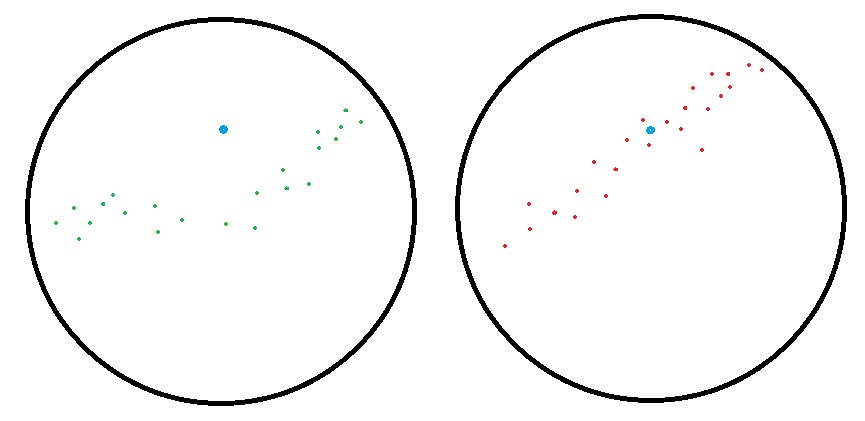
\includegraphics[width=0.4\textwidth]{Path_comp_uncomp}
\caption{The left shows the uncompromised map made up of states avoiding some area and the right shows a compromised map where the states do cross the same area. In this case the state obtained from the particle filter mean, demonstrated in blue, would likely yield a more compromised probability}
\label{fig:compmaps}
\end{figure}
	
A KD tree is used on both maps to find the closest approximate points to each mean found. The few particles gathered by this process are used, by the compromised and uncompromised maps, to form probability density function (PDF) by means of a Kernel density estimation (KDE). This distribution is used to obtain the probability the mean of the particle filter approximation falls within each map. The product of these two probability biases the input to the next iteration to the Bayes equation \ref{fig:Bayes} where b = behavior of the robot, s = state of the robot and c = the probability the robot is compromised.

\begin{equation}
 \beta el =\frac {(P(b,s|c)P(c)} {(P(b,s|c)P(c) + 
 P(b,s|c' )P(c' ))} 
 \label{fig:Bayes}
\end{equation}

This implementation provides a way a way for the change in behavior, that is from uncompromised to compromised or vice versa, to impact the current belief.


\subsection{Distributed State Estimation}
KFs perform better with more inputs. This is the driving force behind increasing the accuracy of mobile robot localization. With more sensor inputs, noise can be removed more accurately. One way to increase the number of sensor inputs to a filter is to add more sensors to the robot. However this will rapidly drive up cost and complexity. Another solution is to have robots share their information about the surrounding world, thus artificially inflating the number of sensors a robot has.

The flow for this system is as follows. A robot at position $p_l$, where $l$ represent that this position is with respect to the local frame, detects another robot at position $g_l$. The robot at $p_l$ then calculates its' pose in with respect to the global frame, $p_g$ and then transforms $g_l \rightarrow g_g$. This position $g_g$ is then shared with the robot's in the surrounding environment, which integrate the position into their own localization estimate. This is summarized in \autoref{tab:external_pose}.

\begin{table}
\centering
\begin{tabular}{c}
KF output $\rightarrow p_l, p_g$ \\
Lidar scan $+ p_l \rightarrow g_l$ \\
$g_g \rightarrow$ KF input
\end{tabular}
\caption{General algorithm for computing external pose.}
\label{tab:external_pose}
\end{table}

The following sections how the position estimates $p_l$, $p_g$, $g_l$, and $g_g$ are obtained. All localization estimates will be referenced with an associated coordinate frame. These frames are described in ROS REP-105 \cite{REP_105}. They are the base\_link (aka base\_footprint) frame, which is rigidly fixed to the center of the robot, the odom (aka local) frame, which is continuous but subject to drift over time, and the map (aka global) frame, which is subject to discrete jumps but does not drift over time.
 
\paragraph{Filters}
There are two filters operating on the robot to create a whole localization estimate. The first is the \textit{Continuous Filter} (CF), and the second is the \textit{Discrete Filter} (DF). They each perform a separate but related localization task, and combined give a full localization estimate with respect to both the local and global frame of the robot. 

\subsubsection{Continuous Filter} \label{con_filter_subsubsection}
The CF calculates the transformation from $odom \rightarrow base\_link$. It receives odometry information from the robot's wheel encoders and IMU. Using this information it publishes the $odom \rightarrow base\_link$ transformation. Another name for the CF is the Self Filter.  

\subsubsection{Discrete Filter} \label{disc_filter_subsubsection}
The DF calculates the transformation from $map \rightarrow base\_link$. Because the ROS TF package that handles coordinate frame transformations enforces a tree structure where each node can only have one parents, the DF references the $odom \rightarrow base\_link$ transform published by the CF and publishes a transform from $map \rightarrow odom$. The inputs to the DF are the robot's wheel encoder odometry, IMU readings, a GPS, and external poses calculated by other robots. Another name for the DF is the Distributed Filter.


\section{Experiments}

The three different concepts were implemented and are detailed below.

\subsection{Secure Ad-Hoc Channel Communication}

In order to communicate between agents within the proximity range the wifi communication channel is analyzed. In order to keep the agent to agent principle we render the IP layer of communication unfit and to a more conservative approach of omitting the IP layer to the network stack.

Use of the data link layer pushed the use of raw sockets; the socket class for python was used instead. The downside however remains in that the socket class requires sudo, or root, access in order to run the node since permissions do not allow sockets to be ran under a regular user. Since giving admin privileges to a node can be considered a threat, there is push to either change the permissions for saw sockets or to change to a new library all together.

The python code was first loaded onto two different laptops, both running Ubuntu 14.04 LTS with a full ROS install, and connectivity was established. We first start with obtaining the database from the 'central base' module created as seen in figure~\ref{fig:TopicIntr1}. The directory where the database file resided was located and moved to the correct agent where the robot\_proxy was executed.

\begin{figure}[]
\centering
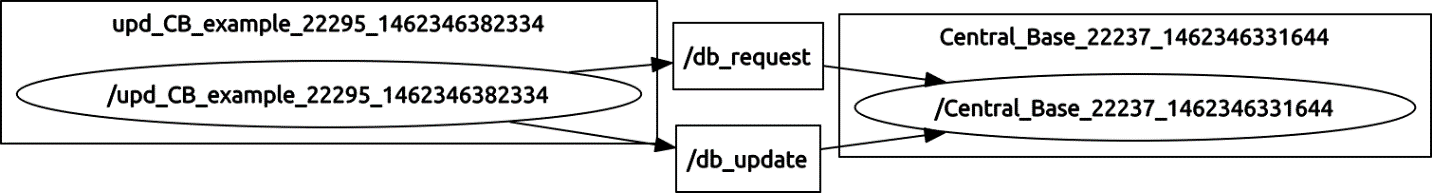
\includegraphics[width=0.4\textwidth]{TopicIntr1}
\caption{The initial communication with the central frame is made here. Each database, in its encrypted form, is created to be placed with each corresponding agent.}
\label{fig:TopicIntr1}
\end{figure}

A new connection is detected and notified via a list in topic /Host\_lists which signifies a working connection. Now, in order to test the appropriate data the testing node Simple\_calc.py was used as seen in Figure~\ref{fig:TopicIntr2}.

\begin{figure}[]
\centering
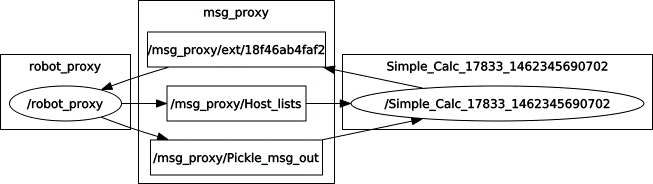
\includegraphics[width=0.4\textwidth]{TopicIntr2}
\caption{Topic Interaction with node- As new agents are populated, the external host lists are updated. Hence, when the topic handler retrieves the Host Lists from all the connection objects, the nodes in the current system will have an accurate overview of which topics are being published elsewhere based on the MAC of each external agent.}
\label{fig:TopicIntr2}
\end{figure}

Pickle\_msg out is the received messages from the outside world that are rebroadcasted. Each external agent connected has a subscriber created through /msg\_proxy/ext/. Scoping is utilized throughout to address each agent outside the current robot. The pickle\_msg contains a MAC field After setting up the correct interface to transfer frames over wifi things behaved like a regular wire. The OS was used in to set up a local network; with the secure nature of the messages exchanged this network can be left open so that future releases will not have difficulty communicating with older models. 

The results were, as expected, the node could not publish another type of message on our specified topic. Then, after making the appropriate PickleSend Type we are able to send the message to the subscriber callback in the robot proxy. From there we learn our transmission was successfully encrypted and transmitted through, received decrypted and unicasted to the receiving host. The process is carried on to the test bench of two zed boards where the implementation of response computation must be extendable to both the laptop and board despite architecture. We are able to verify the authentication and individual agent assignment by verifying the test data itself at each end of the connection.

\subsection{State Detection}
[INSERT RESULTS HERE]

\section{Conclusion}
We have presented three components from a larger chain of trust that is designed to ensure security of not only the agent itself, but also of the group of agents surrounding it.

We have presented a simple distributed state estimation scheme operating over secure network channels that improves the performance of each agent and is augmented with a state detection scheme allowing agents to recognize possible subversive agents in their environment.
% conference papers do not normally have an appendix

% use section* for acknowledgment
\section*{Acknowledgment}
We would like to thank Professors Murat C. Cavusoglu, Russell C. Jackson and Tipakorn Greigarn and for their time, support and guidance.

\printbibliography
\end{document}
